\section[M1: Metamodell]{M1: Meta-Modellierung}
\begin{frame}{Meta-Modellierung}
	\centering
	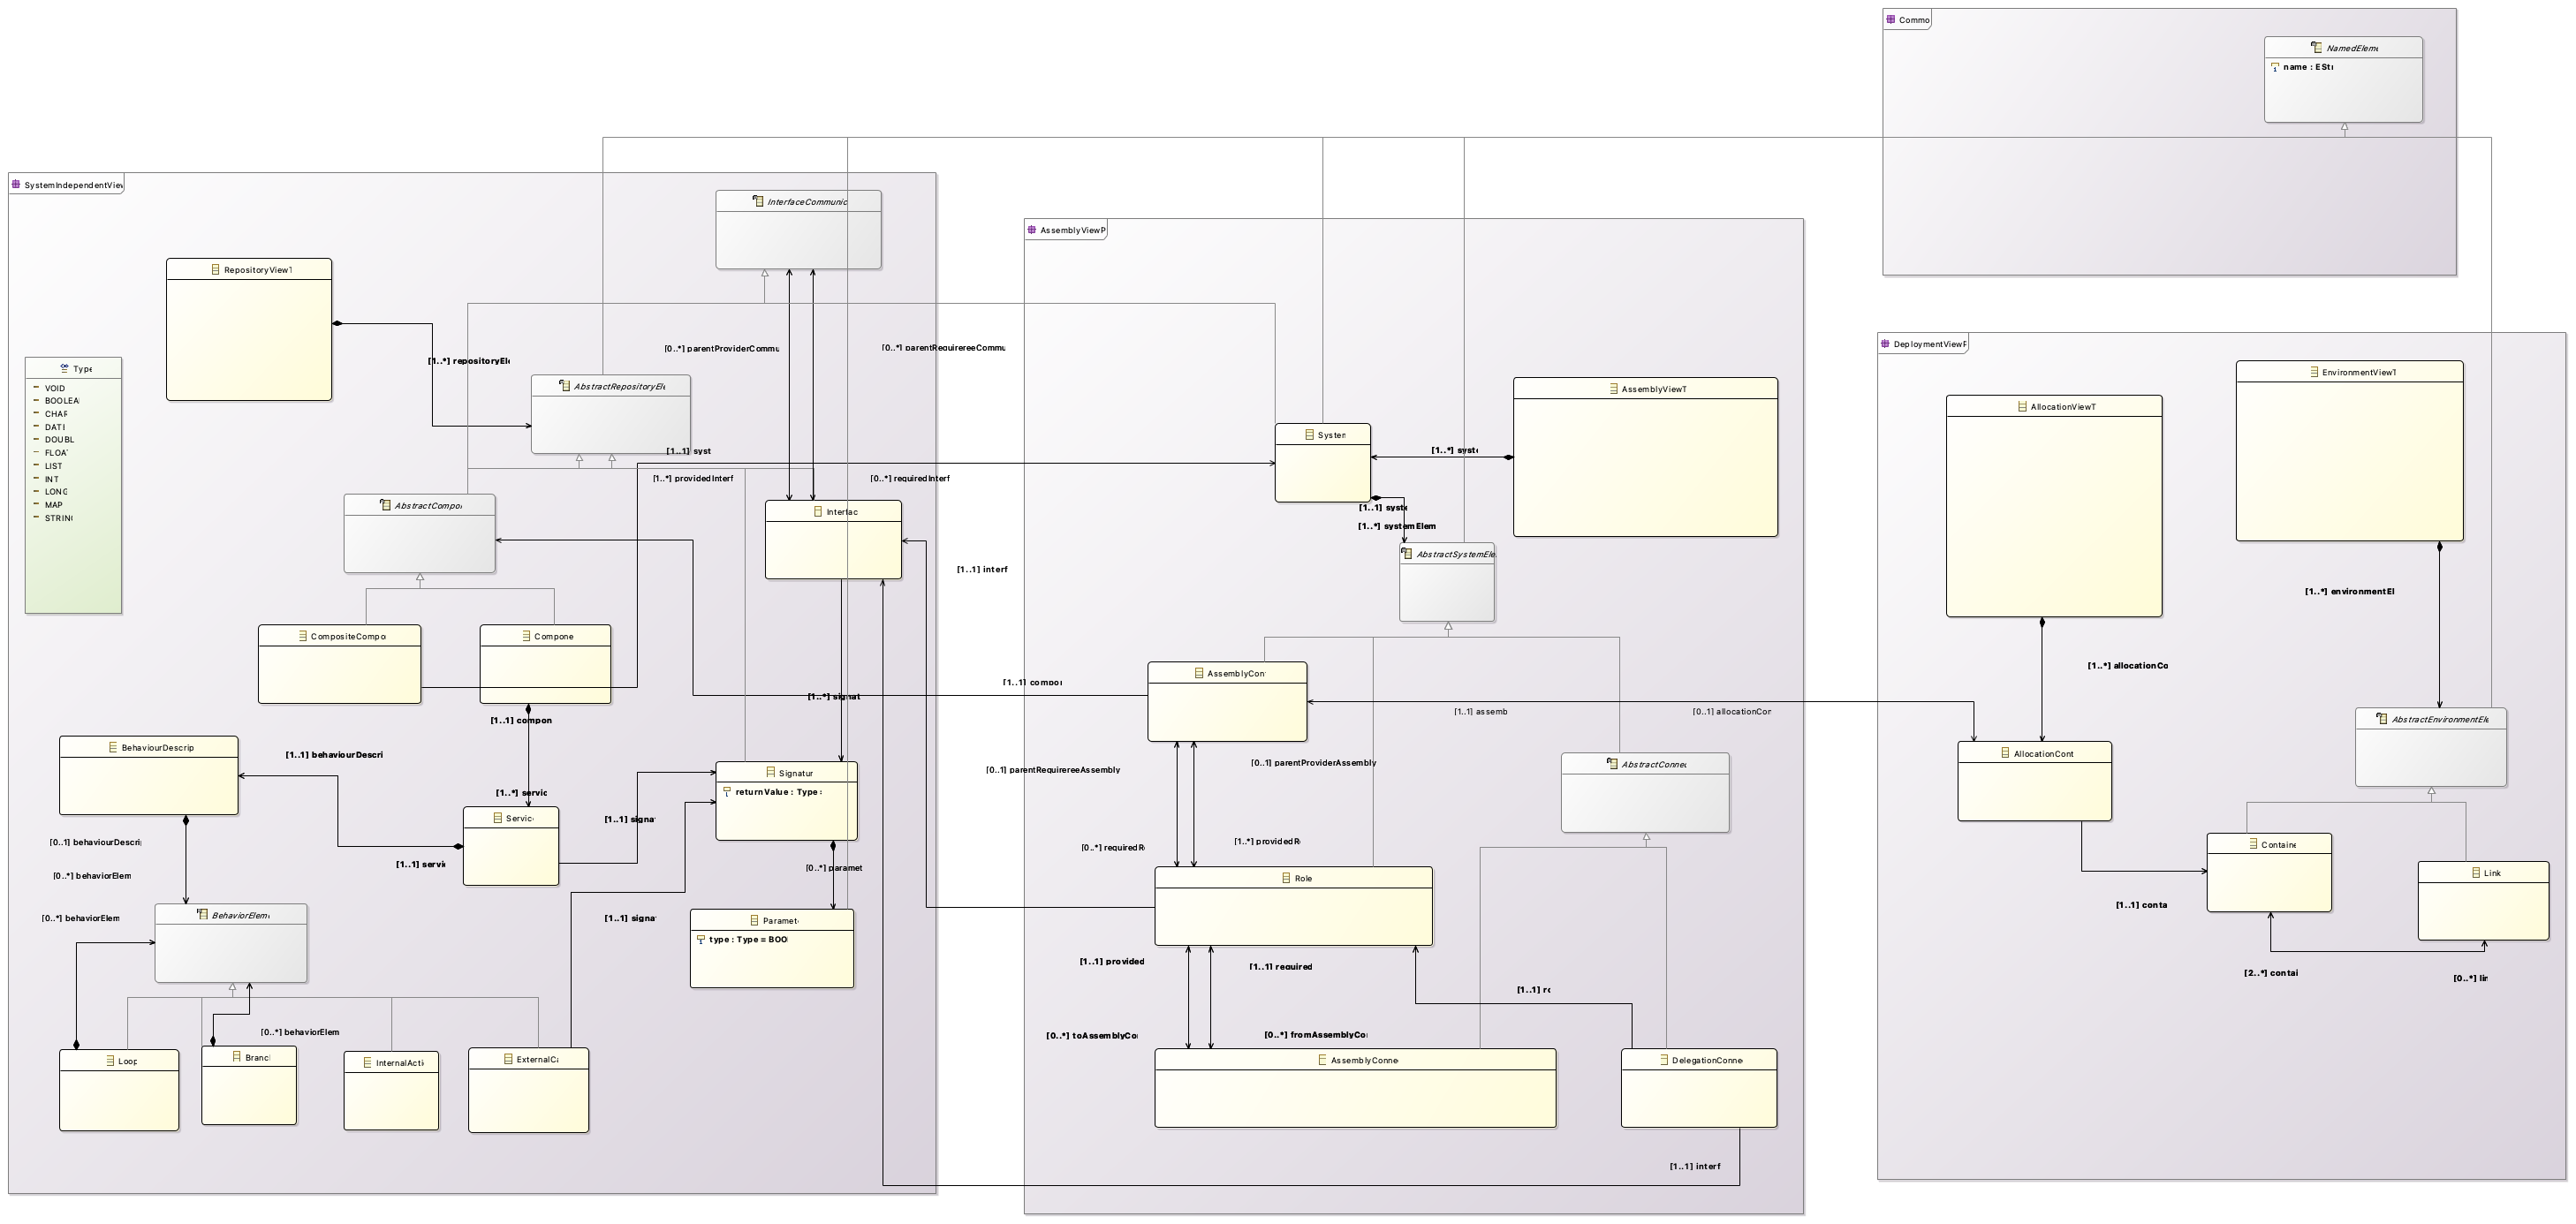
\includegraphics[height=60mm]{figures/meta-modell.png}
\end{frame}

\begin{frame}{Entwurfsentscheidungen für die Meta-Modellierung}
	\begin{enumerate}
		\item Designentscheidung: Verwendung von 4 Packages
		\begin{itemize}
			\item Common Package für wiederverwendbare Elemente
			\item Vorteil: klare Trennung der View Points
			\item Nachteil: geringe Unterstützung für Subpackages von Metamodellen $\Rightarrow$ macht spätere Entwicklung aufwendiger
		\end{itemize}
		\item Designentscheidung: Entscheidung für einfachere Modellierung
		\begin{itemize}
			\item führt zu mehr sowie komplexeren OCL Ausdrücken
			\item erhöht den Bedarf nach bidirektionalen Referenzen
			\item $\Rightarrow$ beeinflusst wie man mit dem Meta-Modell weiterarbeiten kann
		\end{itemize}
		\item Designentscheidung: ENUM zur Modellierung des \texttt{Type}
		\begin{itemize}
			\item Vorteil: einfaches statisches Typesystem
			\item Nachteil: geringe flexibilität $\Rightarrow$ beschränkt den Raum der beschreibbaren Komponenten
		\end{itemize}
	\end{enumerate}
\end{frame}

\begin{frame}{Entwurfsentscheidungen für die Meta-Modellierung}
	\begin{enumerate}
		\setcounter{enumi}{3}
		\item Designentscheidung: Providing/Requiring von Interfaces als Referenz (Set) realisiert
		\begin{itemize}
			\item jedes Interface kann nur einmal in jeder Referenz existieren
			\item Nachteil: geringe Flexibilität $\Rightarrow$ beschränkt den Raum der beschreibbaren Komponenten
		\end{itemize}
	\end{enumerate}
\end{frame}